\section{Desarrollo de la Experiencia.}
\subsection{Trabajo analógico}
\subsubsection{Acondicionamiento de Señal.}
\begin{enumerate}
    \item Ley de Ohm
    \begin{gather}
        V=I\cdot R
    \end{gather}
    \item
        \begin{enumerate}
            \item 
            \item
        \end{enumerate}
        
\end{enumerate}

\subsection{Trabajo digital}
\subsubsection{MSP}
\begin{enumerate}
    \item 
\end{enumerate}

\subsubsection{FPGA}
\begin{enumerate}
    \item 
\end{enumerate}

\begin{figure}[H]
        \centering
        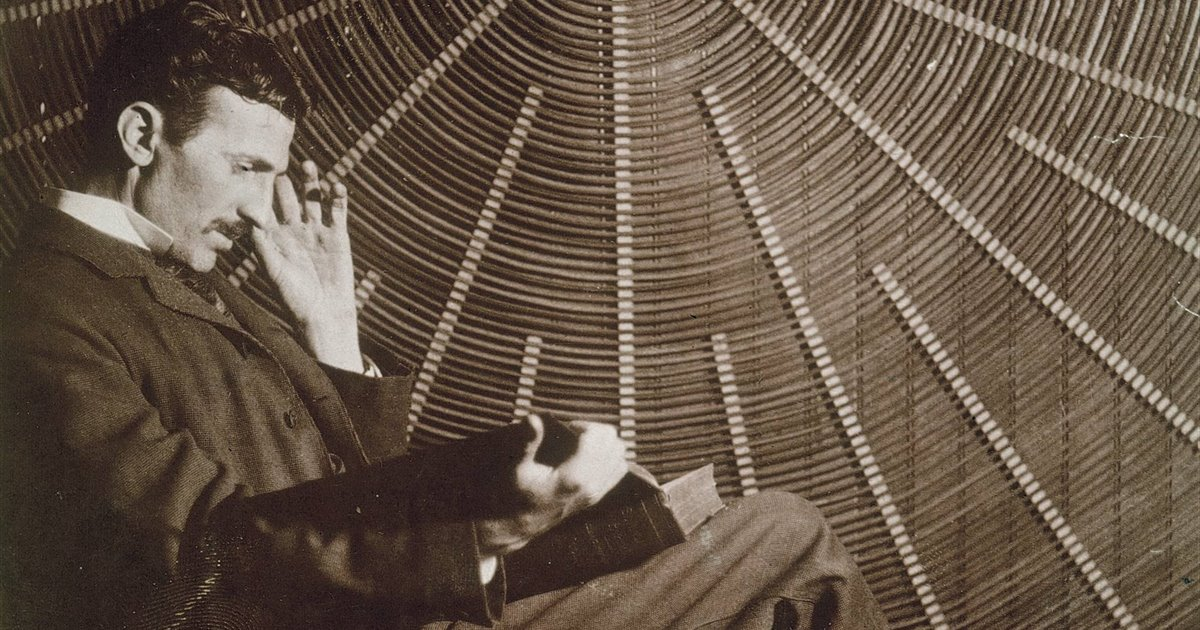
\includegraphics[width=0.8\textwidth]{IMG/Nikola.jpg}
        \caption{Descripción de imagen}
        \label{fig:Imagen1}
 \end{figure}


\newpage
\section{Recordatorios}
\begin{itemize}
    \item Considere todas las posibilidades que ofrece \LaTeX para incluir información. En este documento puede encontrar ejemplos que le serán útiles. Si tienen dudas sobre \LaTeX pueden preguntar también.
    \item Recuerden separar su desarrollo de la experiencia en los puntos de la guía original (lo anterior esta incompleto, pero tiene la idea). 
    \item También, recuerden referenciar sus imágenes (figura \ref{fig:Imagen1}), códigos (anexo \ref{Anexo:Codigo_MATLAB}) y citar \cite{einstein}. 
    \item \textcolor{red}{Existen descuentos por no cumplir con los puntos anteriores.}
    \item Entregue un informe ordenado, que sea fácil de corregir: se sigue el orden de la guía, se explicita que punto se esta respondiendo y demás.
    \begin{align*}
        \text{Informe ordenado} \Rightarrow \text{Fácil de corregir} \Rightarrow \text{Ayudante \Smiley{}} \Rightarrow \text{Mejor nota}
    \end{align*}
